\section{基本知識}
    \subsection{圖是什麼}
    圖 $G$ 由點 $V$ 與邊 $E$ 構成,記做 $G=(V,E)$ 。聽起來很難?

    其實就是像這樣的東西。
    
    \begin{figure}[ht]
        \centering
        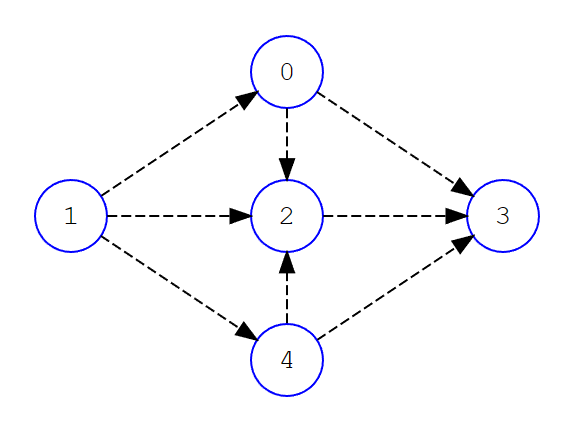
\includegraphics[width=0.5\textwidth]{../Images/Graph1.png}
        \caption{``圖"的示意圖}
    \end{figure}

    \subsection{線上好用工具}

    \url{https://csacademy.com/app/graph_editor/}

    他畫出來的圖長這樣。

    \begin{figure}[ht]
        \centering
        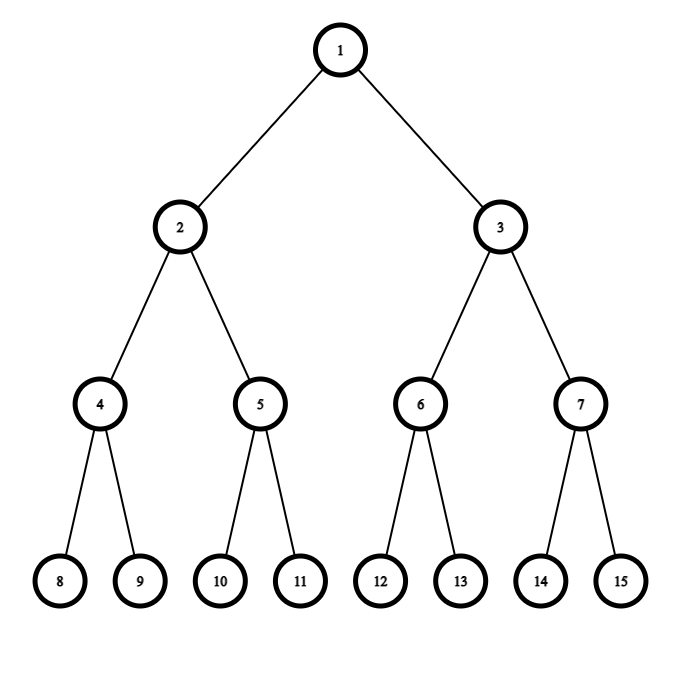
\includegraphics[width=0.5\textwidth]{../Images/Graph2.png}
    \end{figure}

    \subsection{用途}

    所以這就是圖,不過這樣的東西到底會問怎樣的問題呢?

    \example 圖的基本問題
    
    輸入一個有向圖 G 與一個起點 s

    \begin{itemize}
        \item 請計算由 s 出發可以到達的點數(不包含 s)。
        \item 並且計算這些可以到達的點與 s 的距離和。
        \item 假設每個邊的長度均為 1。
        \item 兩點之間可能有多個邊。
        \item 邊的起點與終點未必不同。
    \end{itemize}

    \subsection{存圖}
    \textbf{鄰接串列(Adjacency Link)}

    因為比賽中多數都用不到鄰接矩陣(Adjacency Matrix),所以我先講鄰接串列。

    簡單說就是用 vector 陣列存放點和點之間的關係。

\begin{lstlisting}[caption=存圖]
const int N=100010;
vector<int> g[N];
\end{lstlisting}

    其中,g[x]就是從x出發可以到達的所有點(注意g[x]是一個vector)。
    如果你要新增一個從 a 到 b 的邊,則分為兩種情況。

    \begin{enumerate}
        \item 有向圖 \verb|g[a].push_back(b);|
        \item 無向圖還要加上 \verb|g[b].push_back(a);|
    \end{enumerate}

    會這樣做是因為,無向圖的邊是可以雙向通行的,所以如果a可以到b,
    則b也可以到a。

    \textbf{鄰接矩陣}

    鄰接矩陣使用一個\verb|g[n][n]|表示圖形,其中\verb|g[a][b]>0|表示
    a可以到b,這樣的存圖方式也很直覺,但是會需要花費$O(n^2)$的記憶體空間。
    相較於上一個存圖方式的$O(n+m)$而言會高許多,因為競賽上常常出現$n \le 10^5, \; m \le 2 \times 10^5$
    的情況。

    \subsection{BFS(廣度優先搜索)}
    
    依照到原點所需要經過的邊數由小到大的順序訪問點。以程式來實作的話需要一些簡單的資料結構(queue)。

\begin{lstlisting}[caption=圖的BFS]
vector<int> g[N];
bool isv[N];

void BFS(int s){
    queue<int> q;
    q.push(s);
    
    while(!q.empty()){
        int now=q.front();
        q.pop();
        for(auto e:g[now]) if(!isv[e]){
            q.push(e);
            isv[e]=true;
        }
    }
}
\end{lstlisting}

    不過,如果要解決前面的例題,我們還需要其他東西,幫忙協助計算。

\begin{lstlisting}[caption=圖基本問題題解]
struct info{
    int to,dis;
};
    
vector<int> g[N];
bool isv[N];
    
int bfs(int s){
    queue<info> q;
    q.push({s,0});
    
    int ret=0;
    
    while(!q.empty()){
        info now=q.front();
        q.pop();
        
        ret+=now.dis;
        
        for(auto e:g[now.to]) if(!isv[e]){
            q.push({e,now.dis+1});
            isv[e]=true;
        }
    }
    
    return ret;
}
\end{lstlisting}

    \subsection{DFS(深度優先搜索)}
    跟剛剛BFS走的順序不一樣,在DFS的時候,我們只要有路就一直走,
    直到沒有路我們才考慮上一個有其他路的點。聽起來有點複雜,不過
    程式的寫法與Tree上面的有點像,所以還是很簡單的。

\begin{lstlisting}[caption=圖基本問題題解]
vector<int> g[N];
bool isv[N];
 
void DFS(int n){
    for(auto u:g[n]) if(!isv[u]){
        isv[u]=true;
        DFS(u);
    }
}
\end{lstlisting}

    需要注意的是,isv標記的順序要在DFS往下前,否則如果遇到還就會
    陷入無窮迴圈。

    因為 DFS 明顯比較好寫,因此在可以用 DFS 的情況下幾乎會使用他。

    \subsection{範例與練習}

    \example AP325 P-7-2 開車蒐集寶物

    \textbf{題目敘述}

    參加一個蒐集寶物的遊戲,你拿到一個地圖,地圖上有 n 個藏寶點,
    每個藏寶點有若干價值的寶物,由於你的團隊是最頂尖的,
    只要能到達藏寶點一定可以取得該藏寶點的寶藏。

    從地圖上看得到一共有 m 條道路,每條道路連接兩個藏寶點,
    而且每條道路都是雙向可以通行的。

    在遊戲的一開始,你可以要求直升機將你的團隊運送到某個藏寶點,
    而且你可以獲得一部車與充足的油料,但是直升機的載送只有一次,
    所以你必須決定要從哪裡開始才可以獲得最多的寶藏總價值。

    \textbf{輸入說明}

    第一行是兩個正整數 n 與 m ,代表藏寶地點數與道路數,地點是以 $0$ ~ $n−1$ 編號,

    第二行 n 個非負整數,依序是每一個地點的寶藏價值,每個地點的寶藏價值不超過 $100$ 。

    接下來有 m 行,每一行兩個整數 a 與 b 代表一個道路連接的兩個地點編號。

    n 不超過 $5 \times 10^4$,m 不超過 $5 \times 10^5$ 。

    兩點之間可能有多條道路,有些道路的兩端點可能是同一地點。
    
    \textbf{輸出說明}

    最大可以獲得的寶藏總價值。

    \textbf{範例測試}

    \begin{tabular}{|m{7cm}|m{7cm}|}
        \hline
        範例輸入 1 & 範例輸出 1 \\
        \hline
        \verb|7 6|  & \verb|9| \\
        \verb|5 2 4 2 1 1 8|  & \\
        \verb|5 1|  & \\
        \verb|1 3|  & \\
        \verb|1 4|  & \\
        \verb|2 0| & \\
        \verb|2 0|  & \\
        \verb|3 3|  & \\
        \hline
    \end{tabular}

    \begin{tip}
        通常題目給的圖不一定可以從起點到達所有的點,
        這樣我們會說這個圖是非連通的,反之從起點可以到任何地方的稱為連通圖。
    \end{tip}

    我們可以在DFS的過程中記錄並回傳總價值,所以我們的DFS不再是void,而可以是int
    (或 long long 之類的)。

    因為圖非連通,所以我們需要對每一個點都做確認,並找出所有的連通分量(也就是每一個
    連通的子圖)裡面所有點的總和的最大值。

\begin{lstlisting}[caption=開車蒐集寶物題解]
int val[N];
vector<int> g[N];
bool isv[N];
    
int dfs(int n){
    int ret=val[n];
    for(int next:g[n]){
        if(!isv[next]){
            isv[next]=true;
            ret+=dfs(next);
        }
    }
    return ret;
}
    
int main(){
    // input
    
    int ans=0;
    
    for(int i=0;i<n;++i){
        if(!isv[i]){
            isv[i]=true;
            ans=max(ans,dfs(i));
        }
    }
    
    cout<<ans<<"\n";
}
\end{lstlisting}

    \problem CSES 1192 Counting Rooms

    \textbf{題目敘述}

    給你一張圖,請你算出房間數量。地圖有 $n \times m$ 個格子,
    每一個格子不是地板就是牆壁。你可以往上下左右的地板行走,
    所有依照這個方式走的到的位置都算同一個房間。

    \textbf{輸入說明}

    第一行輸入兩個數字 $n,m$ ,緊接著是 $n$ 行 $m$ 列的字元(字串), \verb|#| 表示牆壁,\verb|.| 表示地板。
    
    \textbf{輸出說明}

    一個整數表示房間數。

    \textbf{範例測試}

    \begin{tabular}{|m{7cm}|m{7cm}|}
        \hline
        範例輸入 1 & 範例輸出 1 \\
        \hline
        \verb|5 8|  & \verb|3| \\
        \verb|########|  & \\
        \verb|#..#...#|  & \\
        \verb|####.#.#|  & \\
        \verb|#..#...#|  & \\
        \verb|########| & \\
        \hline
    \end{tabular}

    \begin{tip}
        可以使用常數陣列表達相對方位,如下:

        \verb|const int dr[]{1,0,-1,0}, dc[]{0,1,0,-1};|
    \end{tip}

    \problem CSES 1193 Labyrinth

    \textbf{題目敘述}

    給你一張圖,請你從 A 走到 B。地圖有 $n \times m$ 個格子,
    每一個格子不是地板就是牆壁。你可以往上下左右的地板行走,
    所有依照這個方式走的到的位置都算同一個房間。

    \textbf{輸入說明}

    第一行輸入兩個數字 $n,m$ ,緊接著是 $n$ 行 $m$ 列的字元(字串),
     \verb|#| 表示牆壁,\verb|.| 表示地板 , A 是起點, B 是終點。
    
    \textbf{輸出說明}

    如果存在路徑,首先輸出``YES",否则打印``NO"。

    如果存在路徑,輸出最短路徑的長度,以及路徑描述,路徑描述是由字元 L(左)、
    R(右)、U(上)和 D(下)组成的字串。可以打印任何有效的解答。

    \textbf{範例測試}

    \begin{tabular}{|m{7cm}|m{7cm}|}
        \hline
        範例輸入 1 & 範例輸出 1 \\
        \hline
        \verb|5 8|  & \verb|YES| \\
        \verb|########|  & \verb|9| \\
        \verb|#.A#...#|  & \verb|LDDRRRRRU| \\
        \verb|#.##.#B#|  & \\
        \verb|#......#|  & \\
        \verb|########| & \\
        \hline
    \end{tabular}

    \problem CSES 1666 Building Roads

    \textbf{題目敘述}

    給你 $n$ 個點 $m$ 條無向邊。
    請你找出要讓這張圖連通的最少所需新增邊數。
    還有給出具體方案。節點編號為 $1 \cdots n$。

    \textbf{輸入說明}

    第一行輸入兩個數字 $n,m$ ,接下來有 $m$ 行,輸入邊 $a_i,b_i$。
    
    保證沒有自環或重邊。

    \textbf{輸出說明}

    第一行輸出需要加上幾條邊,第二行以後給出具體加哪條,如果有多解,
    則輸出任何一個都可以。

    \textbf{範例測試}

    \begin{tabular}{|m{7cm}|m{7cm}|}
        \hline
        範例輸入 1 & 範例輸出 1 \\
        \hline
        \verb|4 2|  & \verb|1| \\
        \verb|1 2|  & \verb|2 3| \\
        \verb|3 4|  &\\
        \hline
    \end{tabular}
    